\section{OOP \& UML}

La fase di implementazione del progetto è stata condotta adottando il paradigma della \textbf{Programmazione Orientata agli Oggetti} (OOP).\
Questo approccio si è rivelato fondamentale per strutturare il codice in modo \textit{modulare}, \textit{manutenibile} e \textit{scalabile},\
in quanto ha permesso di modellare le entità del problema (come i dataset, le sequenze di API e i classificatori) come componenti software interconnesse.\
L'efficacia dell'OOP si fonda su quattro pilastri concettuali:
%... (Lascia qui l'itemize con i 4 pilastri) ...
\begin{itemize}
    \item \textit{Astrazione}: Consente di modellare le entità come classi, focalizzandosi unicamente sugli attributi e sulle interazioni rilevanti per il contesto applicativo,
          nascondendo la complessità sottostante \mycite{oop}.
    \item \textit{Incapsulamento}: Protegge lo stato interno di un oggetto, nascondendolo e consentendo l'interazione con le sue funzionalità per garantirne l'integrità\mycite{oop}.
    \item \textit{Ereditarietà}: Permette di creare nuove astrazioni (sottoclassi) basandosi su astrazioni esistenti (superclassi),
          facilitando il riuso del codice e stabilendo gerarchie logiche tra le classi \mycite{oop}.
    \item \textit{Polimorfismo}: Consente a oggetti diversi di rispondere allo stesso messaggio (chiamata di metodo) in modi specifici alla propria classe,
          permettendo di implementare proprietà o metodi ereditati in forme distinte tra diverse astrazioni \mycite{oop}.
\end{itemize}

Per formalizzare e documentare questa architettura basata sui principi OOP, è stato utilizzato l'\textbf{Unified Modeling Language} (UML)\mycite{ibm_uml}.
Nello specifico, il \textbf{Diagramma delle Classi} è stato scelto per illustrare la struttura del sistema e le relazioni tra i suoi componenti.
Il diagramma delle classi completo che definisce l'architettura logica del progetto è presentato in \autoref{fig:pdfdoc}.

\begin{figure}[htbp] % h=qui, t=top, b=bottom, p=pagina dedicata
    \centering
    % Inserisci la PRIMA pagina del PDF come immagine
    \adjustbox{max width=\linewidth, max height=\textheight}{%
        \includesvg[angle=90]{approccio-proposto/imgs/uml_svg.svg}%
    }
    \caption{Diagramma delle classi UML che descrive l'architettura OOP del sistema.}
    \label{fig:pdfdoc}
\end{figure}

\FloatBarrier

\subsection{Convenzioni e Notazione UML}

Per la corretta interpretazione del Diagramma delle Classi presentato, definiamo le principali convenzioni di notazione UML adottate, relative alla struttura delle classi, alla visibilità e ai tipi di relazioni.

\subsubsection{Struttura della Classe e Simboli di Visibilità}

La classe è l'elemento fondamentale del Diagramma delle Classi.\
Come mostrato in \autoref{fig:uml-classe-convenzioni}, è rappresentata da un rettangolo suddiviso in tre compartimenti che ne definiscono l'identità e il comportamento:
\begin{enumerate}
    \item \textbf{Nome} (Superiore): Contiene il nome della classe.
    \item \textbf{Attributi} (Centrale): Elenca le proprietà della classe.
    \item \textbf{Metodi} (Inferiore): Elenca le operazioni della classe.
\end{enumerate}

Il costrutto tra parentesi angolari (\texttt{$\ll$nome$\gg$}) viene chiamato \textit{stereotipo} e serve ad estendere il vocabolario del UML,\
aggiungendo ulteriori significati (es. \texttt{$\ll$abstract$\gg$} per indicare un elemento astratto o \texttt{$\ll$query$\gg$} per i metodi che non alterano lo stato).

\begin{figure}[h!]
    \centering
    \adjustbox{max width=0.5\textwidth, max height=0.5\textheight}{%
        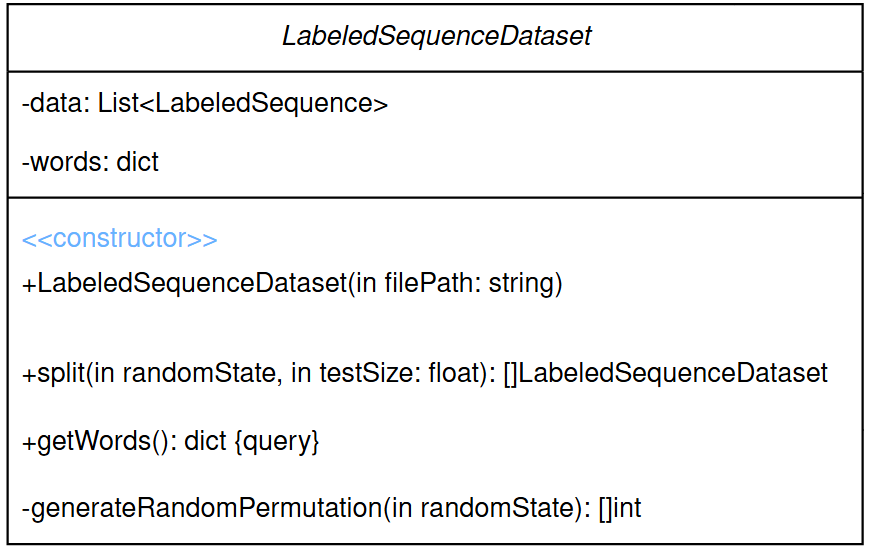
\includegraphics{approccio-proposto/imgs/classe.png}%
    }
    \caption{UML - Classe}
    \label{fig:uml-classe-convenzioni}
\end{figure}

La dichiarazione di un metodo o attributo è preceduta da un simbolo che ne indica la \textbf{visibilità},\
un concetto fondamentale per definire quali elementi possono interagire con l'oggetto.\
In \autoref{tab:visibilita-uml} sono riepilogati i simboli e il loro significato:\

\begin{table}[h!]
    \centering
    \caption{Simboli di visibilità in UML}
    \label{tab:visibilita-uml}
    \begin{tabular}{c l p{8cm}}
        \toprule
        \textbf{Simbolo} & \textbf{Tipo di visibilità} & \textbf{Descrizione}                                    \\
        \midrule
        +                & Pubblica                    & Qualsiasi elemento può accedere                         \\
        -                & Privata                     & Solo la classe stessa ne ha accesso                     \\
        \#               & Protetto                    & Solo la classe e le sue sottoclassi ne hanno accesso    \\
        \textasciitilde  & Package                     & Solo gli elementi dello stesso package ne hanno accesso \\
        \bottomrule
    \end{tabular}
\end{table}

\subsubsection{Definizione di Attributi e Metodi}

La notazione UML stabilisce formati rigorosi per la dichiarazione di attributi e metodi, specificando dettagli come la molteplicità e le proprietà comportamentali.\
La definizione di un attributo segue il formato:
\[
    [\langle \textit{visibilità} \rangle] \;
    \langle \textit{nome} \rangle [\langle \textit{molteplicità} \rangle]: \langle \textit{tipo} \rangle \;
    [= \langle \textit{valore} \rangle][{\textit{proprietà}}]
\]
\textit{Nota: gli elementi tra parentesi quadre [ ] sono opzionali. La visibilità, se non specificata, va intesa come Protetta.}

La \textbf{molteplicità} indica quante istanze\footnote{Un \textbf{istanza} è una instanzazione di una classe, ovvero un oggetto in esecuzione.} sono presenti di quell'attributo;\
se non esplicitata si intende $1$.\
Può essere un range nel formato \textit{min..max}, dove \textit{max} può assumere il valore \textit{*} per indicare l'assenza di un limite.

I valori assumibili dal campo \textit{proprietà} per gli attributi includono: \textbf{changeable} (valore di default), \textbf{addOnly} (solo aggiunte in caso di molteplicità $>1$),\
e \textbf{frozen} (valore immutabile una volta assegnato).

La definizione di un metodo segue invece questo formato:
\[
    [\langle \textit{visibilità} \rangle] \;
    \langle \textit{nome} \rangle
    (\langle \textit{lista parametri} \rangle)
    : \langle \textit{valore di ritorno} \rangle
    [\langle \textit{proprietà} \rangle]
\]
I valori possibili per le proprietà di un metodo includono \textbf{isQuery} (non altera lo stato), \textbf{leaf} (non specializzabile),\
e proprietà relative alla concorrenza come \textbf{sequential}, \textbf{guarded} e \textbf{concurrent}.

\subsubsection{Relazioni Tra Classi}

Le classi nel diagramma UML sono collegate da \textbf{associazioni} che definiscono le loro interazioni.\
Tre tipi di relazioni sono fondamentali in questo progetto:

\paragraph{Composizione (Aggregazione Forte)}
La Composizione (\autoref{fig:uml-composizione}) è una forma forte di associazione che modella la relazione ``parte-intero'' ed è rappresentata da un \textbf{rombo pieno}\\
attaccato alla classe ``intero'' (o contenitore).\
Questa relazione implica che l'esistenza delle ``parti'' dipende strettamente dall'esistenza dell'oggetto ``intero'' e che le parti non possono essere condivise.\
L'esempio mostra come la classe \textit{Sequence} sia composta dalle \textit{ApiCall}, indicando che una sequenza non esiste senza le sue chiamate.

\begin{figure}[h!]
    \centering
    \adjustbox{max width=0.8\textwidth, max height=0.8\textheight}{%
        \includesvg[inkscapelatex=false]{approccio-proposto/imgs/aggregazione.svg}
    }
    \caption{UML - Composizione}
    \label{fig:uml-composizione}
\end{figure}

\paragraph{Use (Dipendenza Implementativa)}
La relazione \textit{use} è formalmente una **Dipendenza** (*Dependency*) ed è rappresentata da una linea tratteggiata con freccia.\
Essa indica una \textbf{dipendenza implementativa} a breve termine: la classe Cliente ha bisogno della classe Fornitore per la sua realizzazione funzionale (e.g., come parametro di un metodo)\
senza conservarne un riferimento strutturale permanente.

\begin{figure}[h!]
    \centering
    \adjustbox{max width=0.8\textwidth, max height=0.8\textheight}{%
        \includesvg[inkscapelatex=false]{approccio-proposto/imgs/use.svg}
    }
    \caption{UML - Use (Dipendenza)}
    \label{fig:uml-use}
\end{figure}

\paragraph{Extends (Ereditarietà)}
La relazione \textit{extends} (\autoref{fig:uml-extends}) è fondamentale per l'OOP.\
Permette alla classe sottoclasse (quella che genera la freccia) di ereditare tutti gli attributi e i metodi della classe padre (quella puntata).\
Questo facilita il riuso del codice e la specializzazione tramite *variazione funzionale* dei comportamenti ereditati.

\begin{figure}[h]
    \centering
    \adjustbox{max width=\linewidth, max height=\textheight}{%
        \includesvg[inkscapelatex=false]{approccio-proposto/imgs/extends.svg}%
    }
    \caption{UML - Extends (Ereditarietà)}
    \label{fig:uml-extends}
\end{figure}

\paragraph{Implements (Realizzazione)}
La relazione \textit{Implements} (\autoref{fig:uml-implements}), rappresentata da una linea tratteggiata con freccia triangolare, descrive la \textbf{realizzazione di un'interfaccia} (o classe astratta).\
La classe che genera la freccia si impegna a implementare tutti i metodi astratti definiti nell'interfaccia puntata.\
Nel nostro diagramma, i classificatori (\texttt{RandomForest} e \texttt{XGBoost}) realizzano un'interfaccia \texttt{$\ll$abstract$\gg$ Classifier} che definisce i metodi \texttt{fit} e \texttt{predict}.

\begin{figure}[h]
    \centering
    \adjustbox{max width=\linewidth, max height=\textheight}{%
        \includesvg[inkscapelatex=false]{approccio-proposto/imgs/implements.svg}%
    }
    \caption{UML - Implements (Realizzazione)}
    \label{fig:uml-implements}
\end{figure}

\paragraph{Package}
I \textbf{package} in UML (\autoref{fig:uml-pacakge}) sono utilizzati per raggruppare logicamente le classi correlate, migliorando l'organizzazione visiva e concettuale del diagramma delle classi.

\begin{figure}[h]
    \centering
    \adjustbox{max width=\linewidth, max height=\textheight}{%
        \includesvg[inkscapelatex=false]{approccio-proposto/imgs/package.svg}%
    }
    \caption{UML - Package}
    \label{fig:uml-pacakge}
\end{figure}

\FloatBarrier